\subsubsection{Diagrama de flujo de datos:}

Refinamos el proceso Consejos del diagrama armazón mediante
una primitiva descendente de descomposición en procesos sin conexiones.\\
Simultaneamente realizamos una descomposición de almacen sobre el
almacén MateDB del armazón.\\
Por último conectamos las descomposiciones resultantes mediante dos
primitivas ascendentes de generación de flujo.\\ 
 
\begin{figure}[H]
\centering
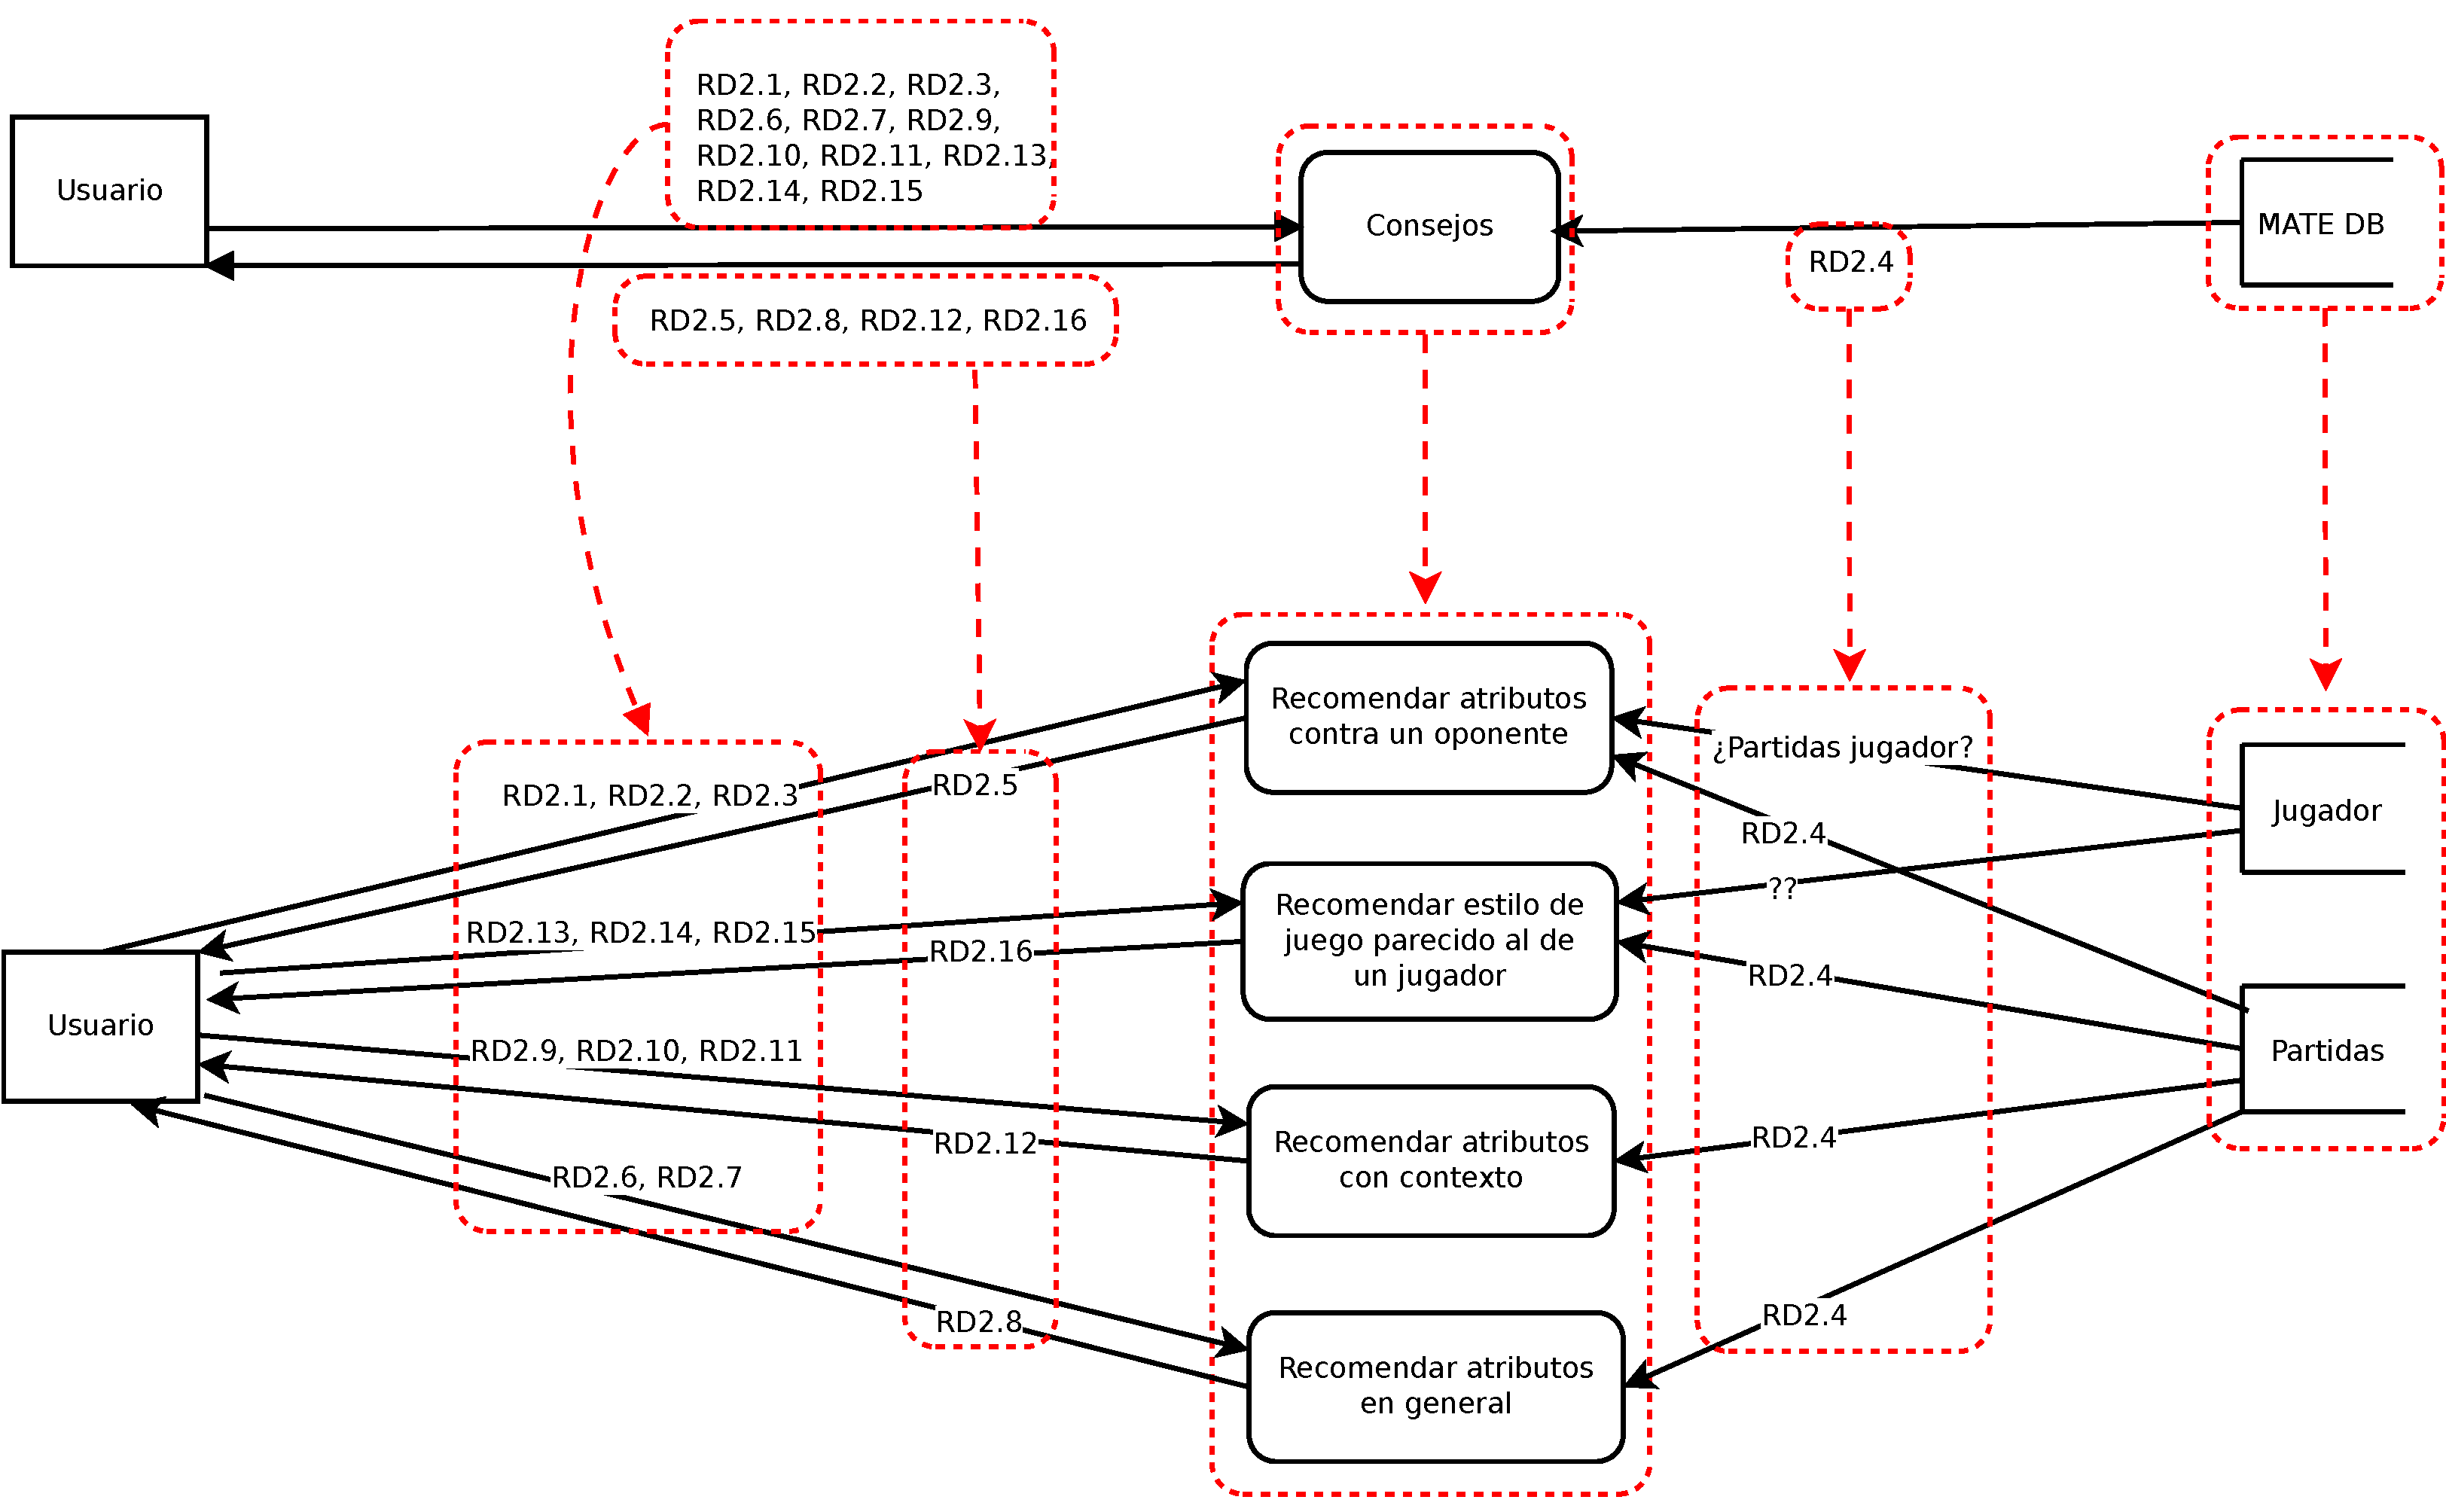
\includegraphics[width=0.7\linewidth]{../Diagramas/pdf/Consejos/RefinamientoConsejos.pdf}
\caption{Flujo de datos del subsistema Consejos}
\end{figure}


\subsubsection{Diagrama externo}

\begin{figure}[H]
\centering
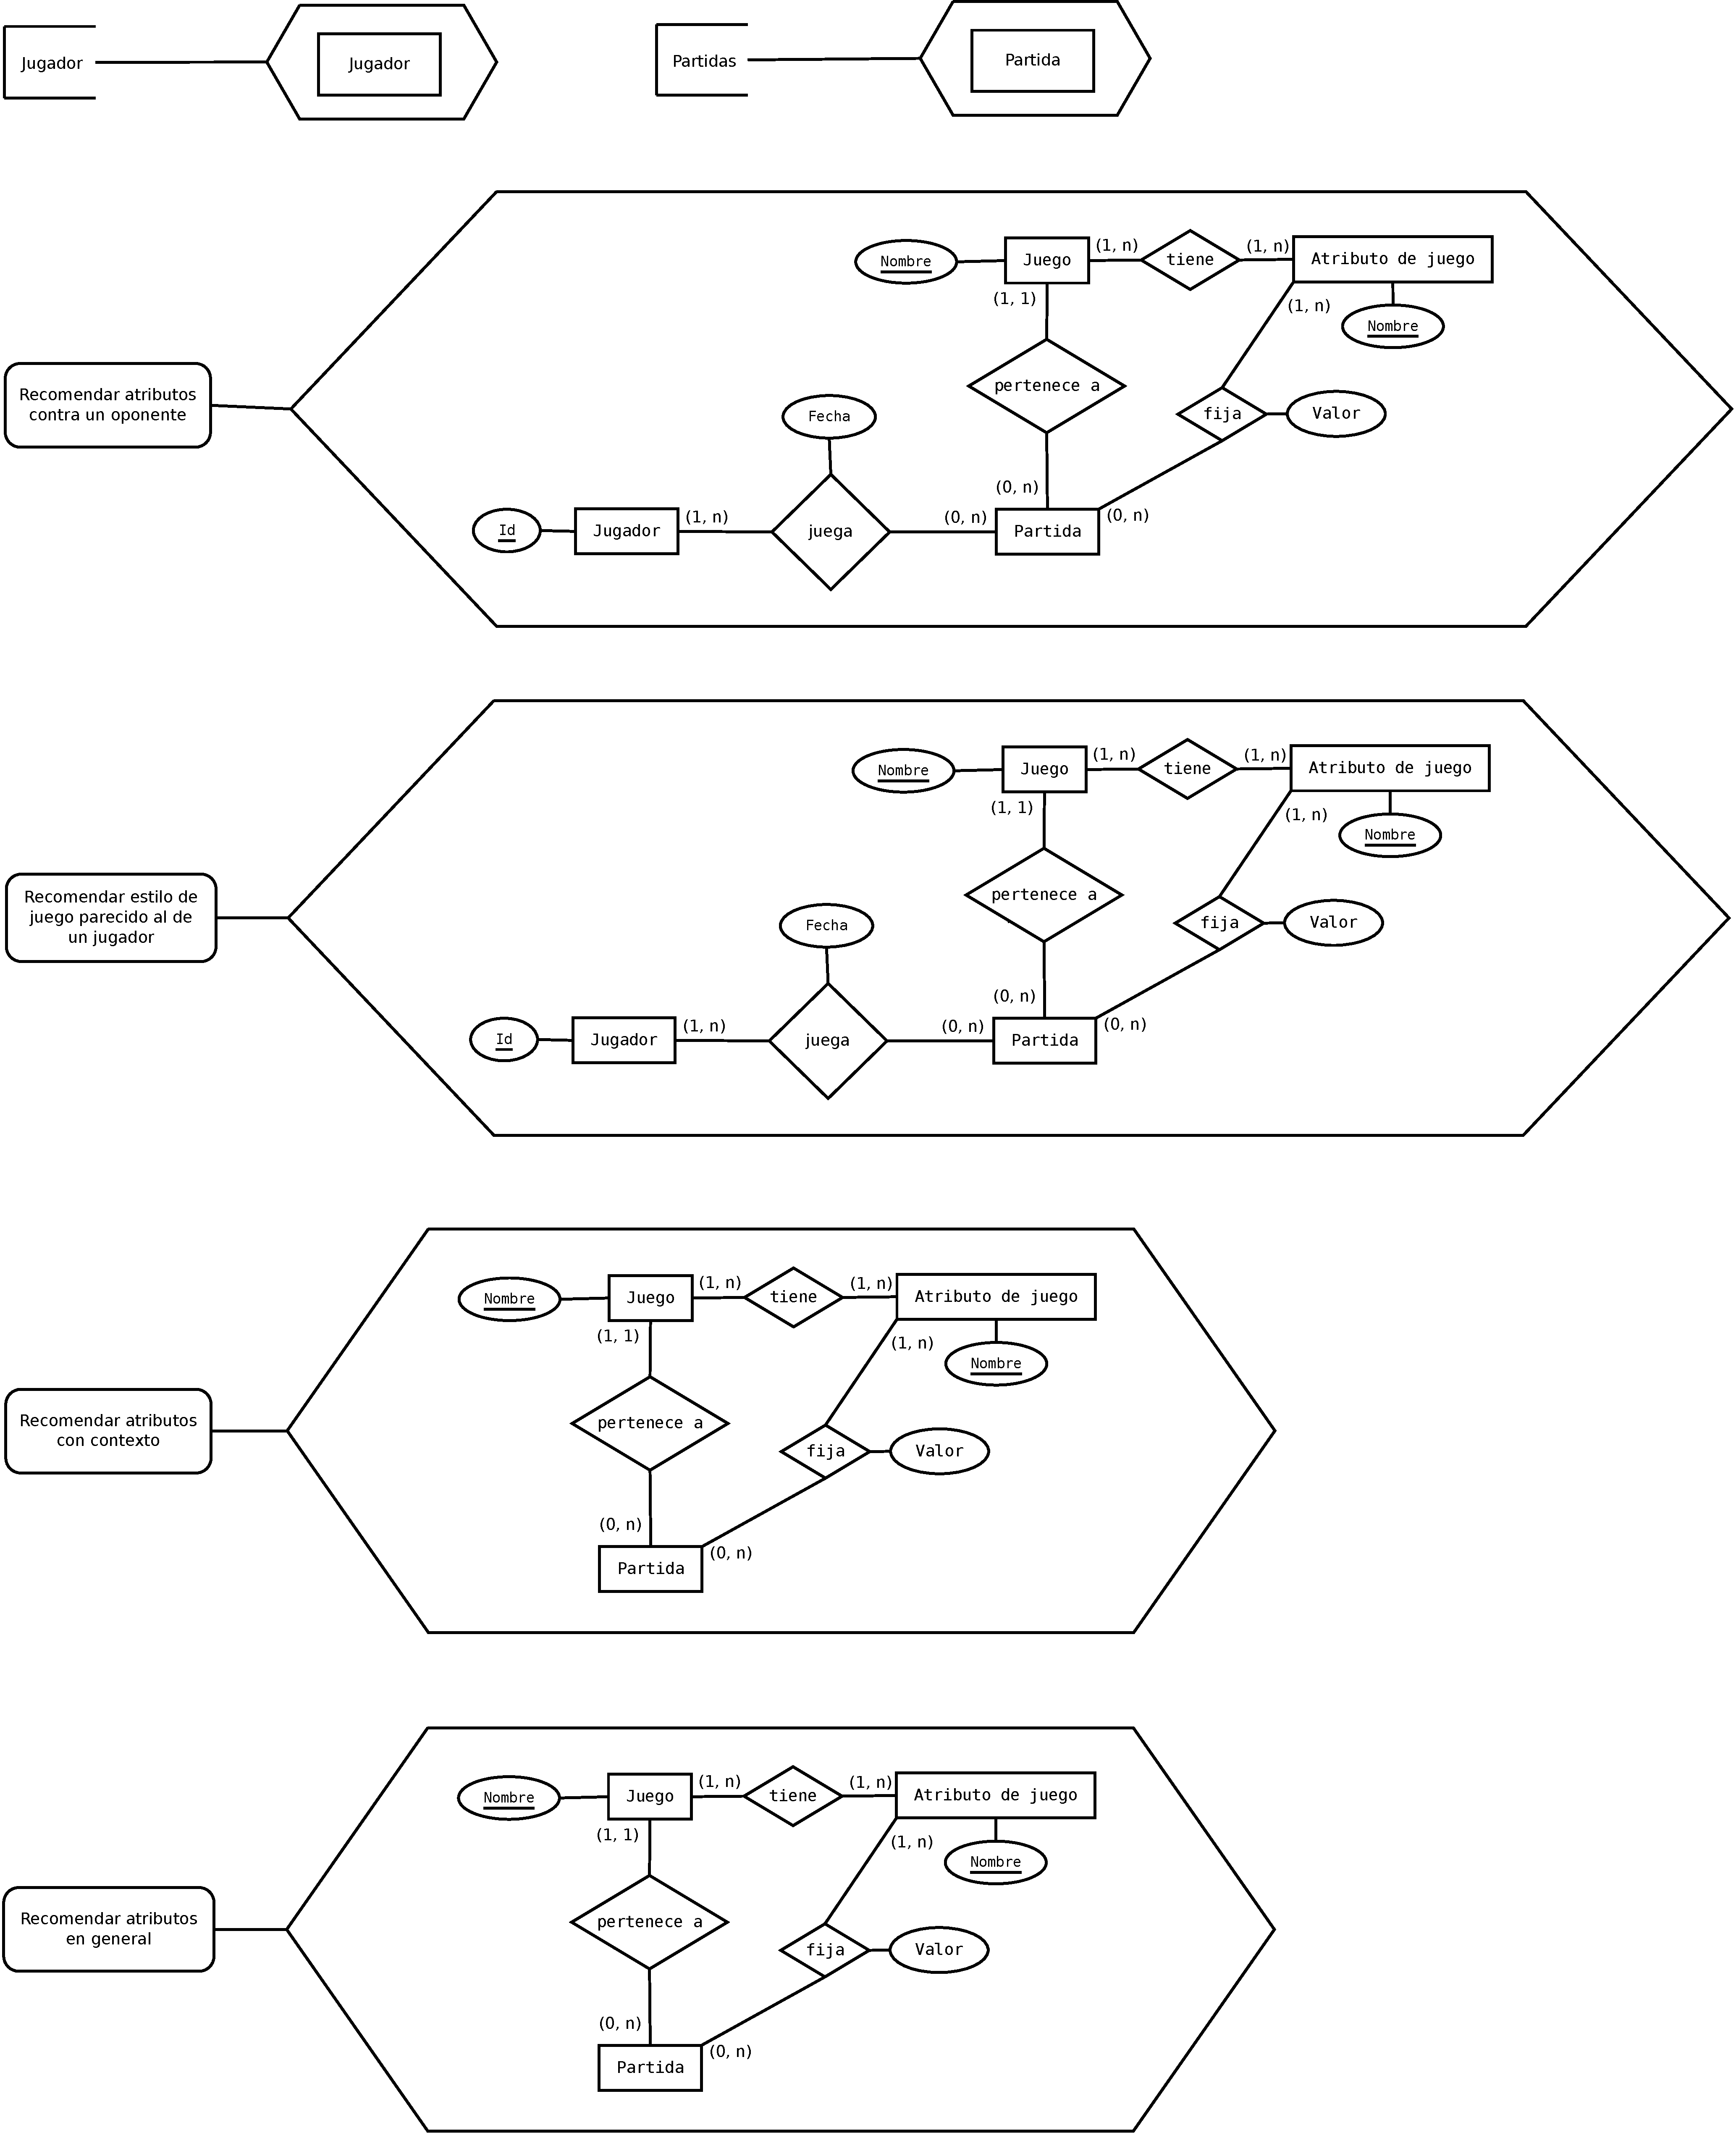
\includegraphics[width=0.7\linewidth]{../Diagramas/pdf/Consejos/ExternoConsejos.pdf}
\caption{Esquema externo del subsistema Consejos}
\end{figure}


\subsubsection{Diagrama E/R}

\begin{figure}[H]
\centering
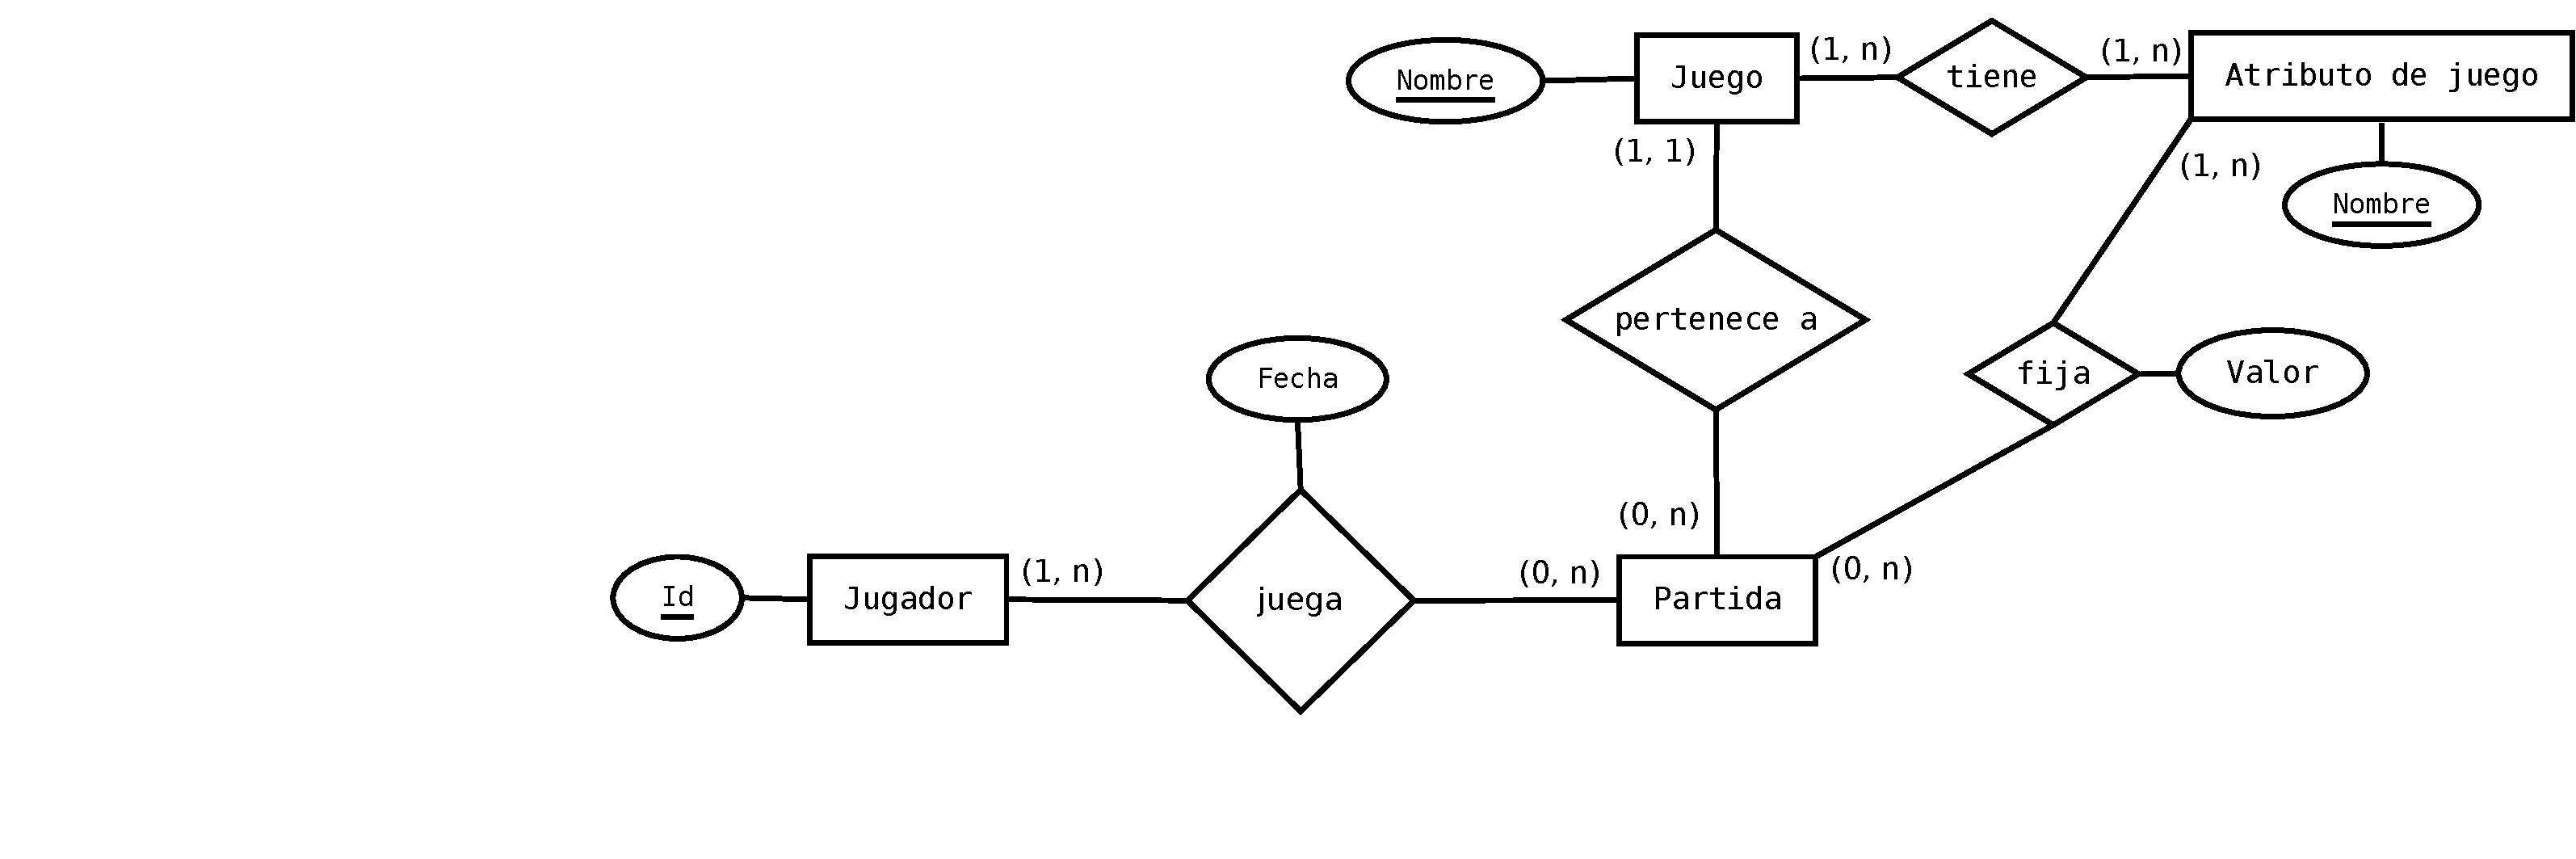
\includegraphics[width=0.9\linewidth]{../Diagramas/pdf/Consejos/ERConsejos.pdf}
\caption{Diagrama E/R del subsistema Consejos}
\end{figure}
